\documentclass[12pt]{article}

\usepackage{sbc-template}
\usepackage{graphicx,url}
\usepackage[utf8]{inputenc}
\usepackage[brazil]{babel}
%\usepackage[latin1]{inputenc}

     
\sloppy

\title{Avaliação de desempenho de implementação paralela do método CSEM 3D no supecomputador Santos Dumont}

\author{Mateus F. Lima de Souza\inst{1,2}, Rômulo T. Lima\inst{1,3}, Roberto P. Souto\inst{1}, \\ 
        Antônio Tadeu A. Gomes\inst{1}, Tiziano Labruzzo\inst{1,4}, Andrea Zerilli\inst{1,4}}

\address{  Laboratório Nacional de Computação Científica (LNCC)\\
  Getúlio Vargas Av., 333, Quitandinha Petrópolis - RJ - Brasil
\nextinstitute
  Centro Federal de Educação Tecnológica Celso Suckow da Fonseca (CEFET-FR) \\
  R. Gen. Canabarro, 485 - Maracanã, Rio de Janeiro - RJ - Brasil
\nextinstitute
Universidade Católica de Petrópolis (UCP)\\
  R. Barão do Amazonas, 124 - Centro, Petrópolis - RJ - Brasil  
\nextinstitute
Zlemlink Ltda \\
Rua Taylor 39, sala 805, Rio de Janeiro-RJ - Brasil  
  \email{\{facanha,romulotl,atagomes,tiziano\}@lncc.br}
}

\begin{document} 

\maketitle

\begin{abstract}
This work presents a parallel execution result in the Santos Dumont supercomputer for an implementation of the CSEM 3D method. Concepts and methods for implementing parallel processing were employed to emphasize the use of computational resources in each node. Thus, it can be verified that there is a limitation in the improvement of performance when increasing the number of computational cores used in the available multicore CPU architecture.
\end{abstract}
     
\begin{resumo} 
Este trabalho apresenta um resultado de execução paralela no supercomputador Santos Dumont para uma implementação do método CSEM 3D. Conceitos e métodos de implementação de processamento paralelo foram empregados para enfatizar o uso de recursos computacionais em cada nó. Assim, pode-se verificar que existe uma limitação na melhoria de desempenho ao aumentar o número de núcleos computacionais utilizados na arquitetura de CPU multicore disponível.
\end{resumo}

\section{Introdução}
Controlled-Source Eletromagnetic (CSEM) é um método de mapeamento geofisico que emprega um monitoramento eletromagnético através de sensores para mapear a resistência elétrica da superfície aquática. Este método é utilizado em larga escala para diversas aplicações, tais como a exploração de hidrocarboneto utilizando tecnologia embarcada. Este trabalho teve como objetivo explorar a eficiência da paralelização MPI do código CSEM 3D~\cite{zerilli2014broadband,zerilli2016broadband}, sendo esta uma implementação em Fortran por diferenças finitas. Outras implementações do método CSEM 3D, por elementos finitos e por volumes finitos (em Python), podem ser consultadas em~\cite{werthmuller_towards_2021}. Como recursos computacionais foram utilizados de 12 até 384 processos MPI no supercomputador Santos Dumont (SDumont).  É apresentada uma análise de desempenho paralelo para dois cenários: utilizando todos os núcleos computacionais e metade deles em cada nó. Percebeu-se uma sensível melhora no desempenho da aplicação com a segunda estratégia.


\section{Metodologia}
\label{sec:metodo}
%
Um diagrama com a arquitetura de CPU multi-core Intel\textregistered~Xeon\textregistered~Gold~6252 disponível entre os nós computacionais Sequana do SDumont é mostrado na Figura~\ref{fig:sequananode}. Cada um destes nós possuem 48 núcleos divididos em 2 sockets contendo 24 núcleos cada. A fim de obter uma análise do comportamento paralelo do código CSEM 3D, foram realizadas execuções paralelas no supercomputador Santos Dumont variando-se de 12 até 384 processos MPI\cite{mpi31}, usando OpenMPI v4.1.2 instalado com compilador GNU v9.3,  organizadas e configuradas conforme mostrado na Tabela~\ref{tab:parallelconfig}. Numa primeira configuração, são utilizados o máximo de 48 núcleos computacionais disponíveis entre os nós computacionais Sequana do SDumont. E em outra configuração, são empregados no máximo 24 núcleos por nó.
%
\begin{figure}
\centering
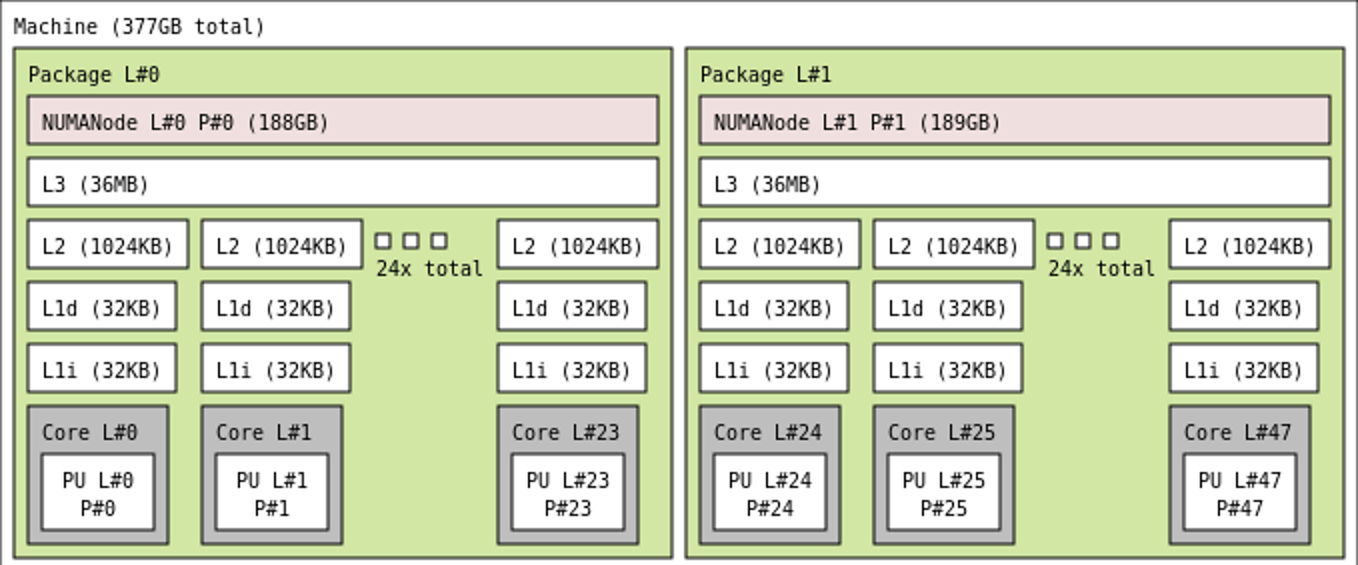
\includegraphics[width=.66\textwidth]{figures/sequanacpudev.png}
\caption{Arquitetura de um nó computacional Sequana no SDumont.}
\label{fig:sequananode}
\end{figure}
%
\begin{table}
\centering
\footnotesize
\caption{Número total de processos MPI, havendo no máximo 48 ou 24 processos MPI por nó, respectivamente nas segunda e terceira colunas.}
\label{tab:parallelconfig}
\begin{tabular}{crr}
\hline
%	&	Máximo de processos MPI por nó	&		\\
\# nós	&	máximo de	&	máximo de	\\
	&	48 MPI/nó	&	24 MPI/nó	\\
\hline
1	&	12	&	12	\\
1	&	24	&	24	\\
1	&	48	&	 -	\\
2	&	96	&	48	\\
4	&	192	&	96	\\
8	&	384	&	192	\\
16	&	 -	&	384	\\
\hline
\end{tabular}
\end{table}

\section{Resultados}
%
O tempos de execução paralela obtidos podem ser visualizados na Figura~\ref{fig:perfpernode}, onde observa-se que o uso de todos nos núcleos em cada nó não resultou necessariamente em um melhor desempenho da aplicação. Pelo contrário, invariavelmente o tempo de processamento foi menor ao se utilizar 24 processos MPI por nó, quando comparado com 48 processos MPI por nó.
É necessário realizar-se um estudo mais detalhado e aprofundado para descobrir as causas deste comportamento, e verificar a possibilidade de obter um efetivo ganho de desempenho utilizando-se todos os núcleos disponíveis em cada nó.
%
\begin{figure}[ht]
\centering
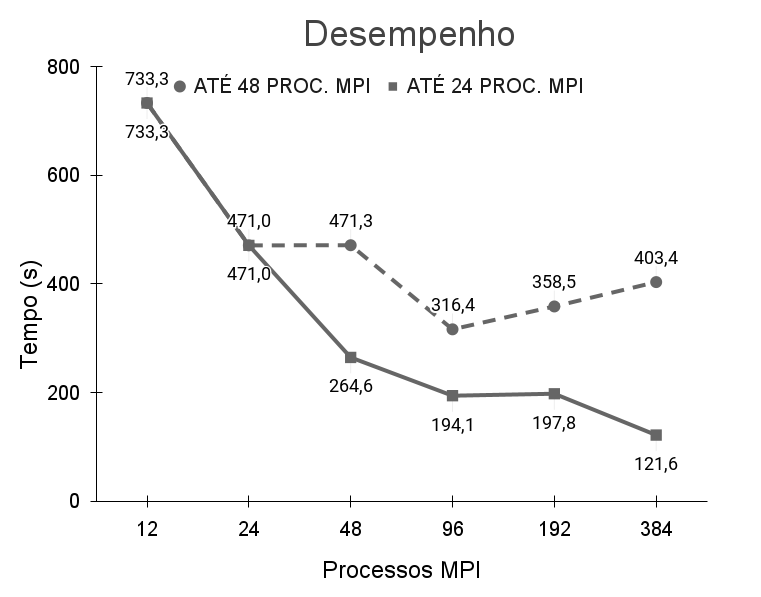
\includegraphics[width=.5\textwidth]{figures/perfpernode.png}
\caption{Tempo de processamento paralelo com até 384 processos MPI, usando no máximo 48 processos MPI por nó (linha tracejada), e no máximo 24 processos MPI por nó.}
\label{fig:perfpernode}
\end{figure}


\section{Comentários}
O estudo de desempenho apresentado neste trabalho mostrou que, para a arquitetura disponível no SDumont, o código paralelo CSEM 3D requer uma investigação mais detalhada para poder melhor entender a limitação observada na melhoria do desempenho paralelo ao se empregar todos os núcleos computacionais do nó. Pretende-se também verificar se este comportamento reproduz-se em outras arquiteturas computacionais de CPU multi-core, tais como a dos processadores AMD EPYC\texttrademark. Uma outra abordagem a ser pesquisada é o emprego de paralelismo em mais de um nível, através do uso paralelização em memória compartilhada com OpenMP~\cite{OpenMP}.


\section*{Agradecimentos}
Os autores agradecem a Petróleo Brasileiro S.A. pelo apoio à pesquisa por meio do Termo de Colaboração número 0050.0121778.22.9. Os autores também agradecem ao Laboratório Nacional de Computação Científica (LNCC/MCTI) por fornecer recursos do supercomputador SDumont, que contribuíram para os resultados da pesquisa relatados neste artigo. \textbf{\url{http://sdumont.lncc.br}}.

\bibliographystyle{sbc}
\bibliography{sbc-template}

\end{document}
